%
% $Id: $
%
%
% Compilar a .pdf con LaTeX (pdflatex)
% Es necesario instalar Beamer (paquete latex-beamer en Debian)
%

%
% Gr�ficos:
% Los gr�ficos pueden suministrarse en PNG, JPG, TIF, PDF, MPS
% Los EPS deben convertirse a PDF (usar epstopdf)
%

\documentclass{beamer}
\usetheme{Warsaw}
%\usebackgroundtemplate{\includegraphics[width=\paperwidth]{format/libresoft-bg.png}}
%\usepackage[spanish]{babel}
\usepackage[latin1]{inputenc}
\usepackage{graphics}
\usepackage{amssymb} % Simbolos matematicos
\usepackage{url}

%\definecolor{libresoftgreen}{RGB}{162,190,43}
%\definecolor{libresoftblue}{RGB}{0,98,143}

%\setbeamercolor{titlelike}{bg=libresoftgreen}

%% Metadatos del PDF.
\hypersetup{
  pdftitle={The Europe Code Week (CodeEU) initiative: Shaping the skills of future engineers},
  pdfauthor={J. Moreno-Le�n, Gregorio Robles},
  pdfcreator={GSyC/LibreSoft \\ Universidad Rey Juan Carlos},
  pdfproducer=PDFLaTeX,
  pdfsubject={CodeEU, CodeWeek, Coding, Programming, CS promotion},
}
%%

\begin{document}

\title{The Europe Code Week (CodeEU) initiative}
\subtitle{Shaping the skills of future engineers}
\institute{jesus.moreno@programamos.es, grex@gsyc.urjc.es \\
GSyC/Libresoft, Universidad Rey Juan Carlos}
\author{J. Moreno-Le�n, Gregorio Robles}
\date{EDUCON 2015, Tallinn, March 19\textsuperscript{th} 2015}%FIXME comprobar la fecha en el programa definitvo

\frame{
\maketitle
\begin{center}
\includegraphics[width=2cm]{format/libresoft-logo}
\hspace{0.5cm}
\includegraphics[width=5cm]{format/gsyc-urjc}
\vspace{0.5cm}
\includegraphics[width=3cm]{format/emadrid.png}
\end{center}
}


% Si el titulo o el autor se quieren acortar para los pies de p�gina
% se pueden redefinir aqu�:
%\title{Titulo corto}
%\author{Autores abreviado}

%% LICENCIA DE REDISTRIBUCION DE LAS TRANSPAS
\frame{
~
\vspace{3cm}

\begin{flushright}
\includegraphics[width=2.2cm]{figs/by-sa}

{\tiny
(cc) 2015 J. Moreno-Le�n and Gregorio Robles \\
  Some rights reserved. This work licensed under Creative Commons \\
  Attribution-ShareAlike License. To view a copy of full license, see \\
  http://creativecommons.org/licenses/by-sa/3.0/ or write to \\
  Creative Commons, 559 Nathan Abbott Way, Stanford, \\
  California 94305, USA. \\
\ \\
Some of the figures have been taken from the Internet \\
Source, and author and licence if known, is specified. \\
For those images, \emph{fair use} applies.
}
\end{flushright}
}
%%

\section{EDUCON 2015 - eMadrid Session}


%--------------------------------------------------------
\usebackgroundtemplate{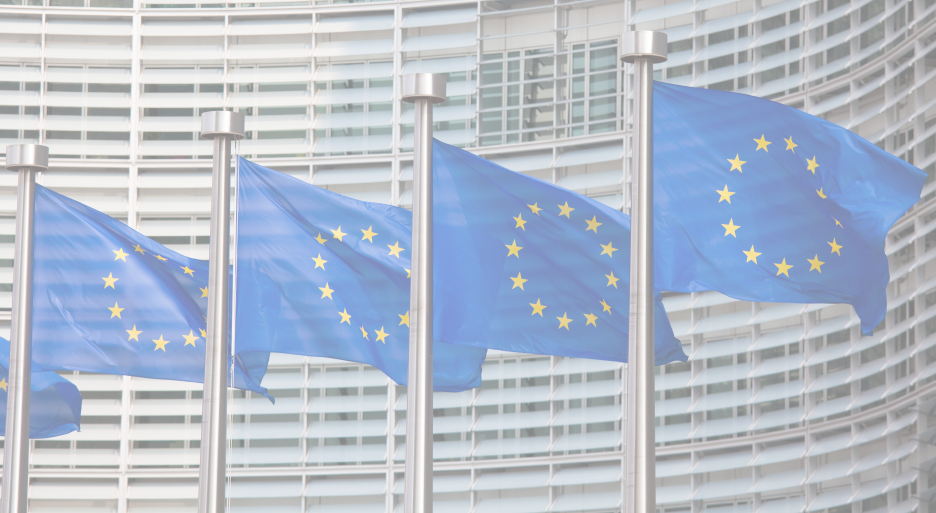
\includegraphics[width=18cm]{figs/eucommission.jpg}}

\begin{frame}
\frametitle{Goal of our paper}

\begin{center}
\Huge {\bf Review CodeEU first editions, share the lessons learned and present suggestions for future initiatives}
\end{center}
\hfill{\Tiny Background picture: http://finances.com}
\end{frame}


%-----------------------    ---------------------------------
\usebackgroundtemplate{\includegraphics[width=14cm]{figs/audience.png}}
% http://cdn.netrafic.com/wp-content/uploads/2011/02/audience.gif

\begin{frame}
\frametitle{Audience}

Who should/could be interested in this talk?

\begin{itemize}
  \item Organizers of CS promotion events
  \item Politicians
  \item CS educators
  \item CS Students
\end{itemize} 

\end{frame}

\usebackgroundtemplate{}
%--------------------------------------------------------
%\usebackgroundtemplate{
\includegraphics[width=13cm,height=9.2cm]{figs/codeweek2.png}}
\begin{frame}
\frametitle{CodeEU Objectives}

\begin{columns}[T]
    \begin{column}{0.87\textwidth}
     \begin{block}{Get addressed the mismatch in digital skills in the European labour market...}
\begin{itemize}
  \item ... making ICT careers more attractive
  \item ... promoting CS among girls
  \item ... modificating CS teaching in K-12
\end{itemize}
    \end{block}
    \end{column}
\end{columns}
\end{frame}

\usebackgroundtemplate{}

%--------------------------------------------------------
%\usebackgroundtemplate{\includegraphics[width=13cm,height=9.2cm]{figs/kids.jpeg}}
\begin{frame}
\frametitle{Why CodeEU}

\begin{figure}[t!]
\begin{center}
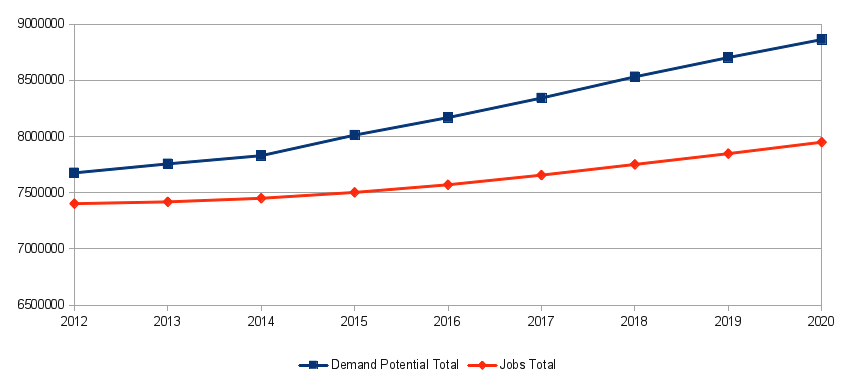
\includegraphics[width=11cm, height=6cm]{figs/Forecast.png}
\end{center}
\label{fig:forecast}
\end{figure}

\begin{center}
Main forecast scenario for ICT jobs and ICT jobs demand in EU
Source: eSkills for Jobs 2014
\end{center}

\end{frame}

\usebackgroundtemplate{}

%--------------------------------------------------------
%\usebackgroundtemplate{\includegraphics[width=13cm,height=9.2cm]{figs/plugins.png}}
% background: http://25.media.tumblr.com/b83aa72682992ab34b8ce7e61c0cb7f9/tumblr_menxc7qcq61ryin08o1_r1_1280.jpg
\begin{frame}
\frametitle{CodeEU Facts}

\begin{figure}[t!]
\begin{center}
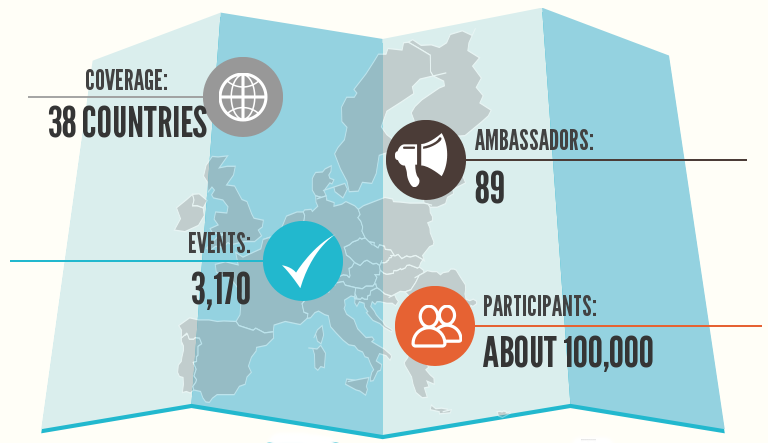
\includegraphics[width=11cm, height=6cm]{figs/facts.png}
\end{center}
\label{fig:facts}
\end{figure}

\begin{center}
Source: CodeWeekEU 2014 factsheet. Alessandro Bogliolo.
\end{center}

\end{frame}

\usebackgroundtemplate{}

%--------------------------------------------------------
%\usebackgroundtemplate{\includegraphics[width=13cm]{figs/iceberg.jpg}}
% background: http://www.wim-network.org/wp-content/uploads/2012/04/iceberg.jpg

\begin{frame}
\frametitle{CodeEU Events}

\begin{figure}[t!]
\begin{center}
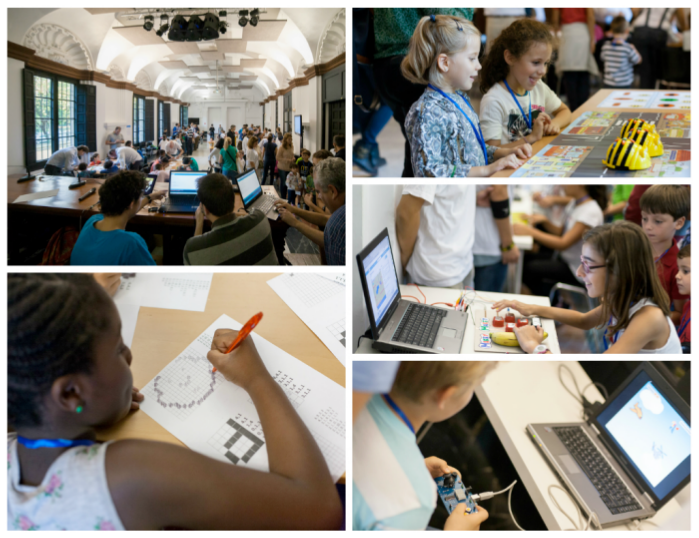
\includegraphics[width=10cm, height=6cm]{figs/codesevilla.png}
\end{center}
\label{fig:facts}
\end{figure}

\begin{center}
Code Sevilla: let's code!
\end{center}

\end{frame}

%--------------------------------------------------------
\begin{frame}
\frametitle{CodeEU Events}

\begin{figure}[t!]
\begin{center}
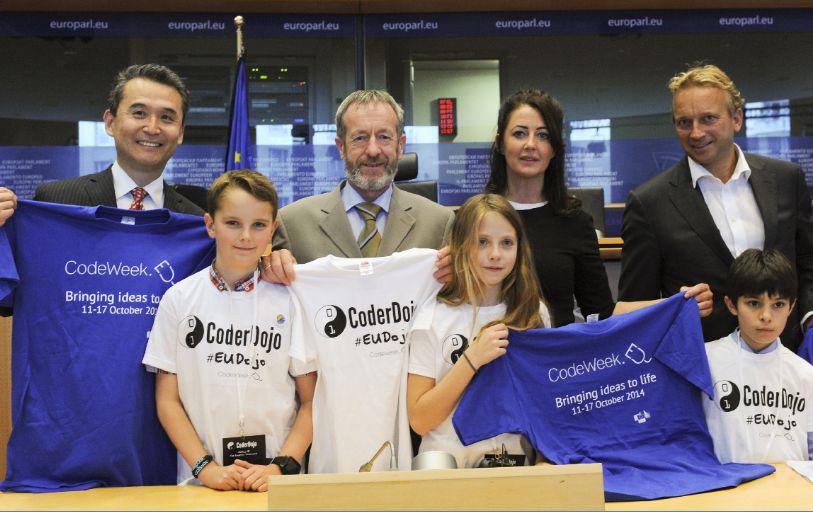
\includegraphics[width=10cm, height=6cm]{figs/coderdojo.png}
\end{center}
\label{fig:facts}
\end{figure}

\begin{center}
Special coding session at EU Parliament
\end{center}

\end{frame}


%--------------------------------------------------------
\begin{frame}
\frametitle{CodeEU Events}

\begin{figure}[t!]
\begin{center}
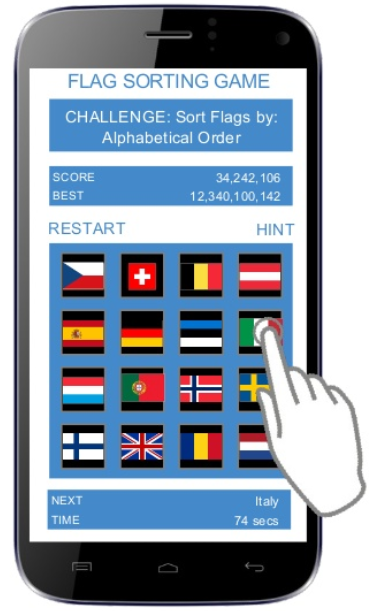
\includegraphics[width=4cm, height=6cm]{figs/flagship.png}
\end{center}
\label{fig:facts}
\end{figure}

\begin{center}
The FlagShip Game: educational crowdcoding \\
http://flagshipgame.eu/
\end{center}

\end{frame}
%--------------------------------------------------------
\begin{frame}
\frametitle{Lessons Learned}
\begin{columns}[T]
    \begin{column}{0.5\textwidth}
    \begin{block}{From 1\textsuperscript{st} edition}
      \begin{itemize}
       \item Support of the government to get to more communities
       \item Media coverage to spread the word about the initiative
       \item Partner with leader companies
      \end{itemize}
    \end{block}
    
    \end{column}
    \begin{column}{0.5\textwidth}
    \begin{block}{From 2\textsuperscript{nd} edition}
    \begin{itemize}
       \item The work cannot be handled by unpaid volunteers
       \item A legal entity is required
       \item How to assess the real impact?
      \end{itemize}
    \end{block}
    \end{column}
  \end{columns}

\end{frame}

%--------------------------------------------------------
%\usebackgroundtemplate{\includegraphics[width=13cm]{figs/take-away.jpg}}
% background: http://2.bp.blogspot.com/-78Eh4TBpdtU/UPw7ULV73PI/AAAAAAAAHAE/6DQfvPNCo-Y/s1600/8723052-stylized-red-stamp-showing-the-term-take-away-all-on-white-background.jpg
\usebackgroundtemplate{\includegraphics[width=13cm]{figs/future.png}}

\begin{frame}
\frametitle{Future Work}
\begin{center}
 \Huge {\bf Create an organization working the year round to get that every week is a code week}
\end{center}
\vspace{\baselineskip}
\vspace{\baselineskip}
\hfill{\Tiny Background picture: Simon Cunningham }

\end{frame}

%--------------------------------------------------------
%\begin{frame}
%\frametitle{GSyC/LibreSoft}

%\begin{figure}[t!]
%\begin{center}
%\includegraphics[width=11cm]{figs/libresoft.jpg}
%\end{center}
%\label{fig:libresoft}
%\end{figure}

%\begin{center}
%The GSyC/LibreSoft research team at URJC (Madrid).
%\end{center}

%\end{frame}

%--------------------------------------------------------
%\begin{frame}
%\frametitle{Our work at GSyC/LibreSoft}

%\begin{figure}[t!]
%\begin{center}
%\includegraphics[width=2.5cm]{figs/research}
% http://www.memphis.edu/crow/images/research_2.jpg
%\hspace{0.1cm}
%\includegraphics[width=2.5cm]{figs/teaching}
% http://2.bp.blogspot.com/_uxgwfriLwSo/TOWDr8IjaLI/AAAAAAAABLM/d7H-G5jIq-c/s1600/teaching.gif
%\hspace{0.1cm}
%\includegraphics[width=2.5cm]{figs/development}
% http://www.vidadigitalradio.com/wp-content/uploads/2009/04/hackers_cartoons.jpg
%\hspace{0.1cm}
%\includegraphics[width=2.5cm]{figs/promotion}
% http://bloggeate.com/wp-content/uploads/2011/04/como-promocionar-tu-blog.jpg
%\end{center}
%\label{fig:whatwedo}
%\end{figure}

%\begin{center}
%GSyC/LibreSoft's tasks: research, teaching, development, promotion of free software.

%\end{center}
%\end{frame}

\usebackgroundtemplate{}

%--------------------------------------------------------
\frame{
\maketitle
\begin{center}
\includegraphics[width=2cm]{format/libresoft-logo}
\hspace{0.5cm}
\includegraphics[width=5cm]{format/gsyc-urjc}
\vspace{0.5cm}
\includegraphics[width=3cm]{format/emadrid.png}
\end{center}
}

\end{document}
